\documentclass[conference]{IEEEtran}
\IEEEoverridecommandlockouts
% The preceding line is only needed to identify funding in the first footnote.

% ---------- packages ----------
\usepackage[T1]{fontenc}
\usepackage{cite}
\usepackage{amsmath,amssymb,amsfonts}
\usepackage{graphicx}
\usepackage{booktabs}
\usepackage{multirow}
\usepackage{textcomp}
\usepackage{xcolor}
\usepackage{url}

\graphicspath{{figures/}}

% Prevent IEEEtran hyphenation warnings on a few long tokens.
\hyphenation{Re-gres-sion-TM}

\begin{document}

\title{Teacher-Guided Knowledge Distillation for the\\
Regression Tsetlin Machine: When, Where, and Why It Helps}

\author{\IEEEauthorblockN{Rupsa Saha}
\IEEEauthorblockA{\textit{Centre for Artificial Intelligence Research (CAIR)} \\
\textit{University of Agder}\\
Grimstad, Norway \\
rupsa.saha@uia.no}}

\maketitle

\begin{abstract}
Regression with the Tsetlin Machine (RegressionTM) is interpretable but typically
requires densely sampled training data, raising the question of how well it can be
trained when data is scarce. We study teacher--student knowledge distillation for
RegressionTM, in which a frozen, better-informed teacher acts inside the student's
training loop: at each sample it adjusts the student's per-sample error before the
Type~I/Type~II feedback decision, steering the clause-level update directly. We develop a
family of such mechanisms and evaluate them under a masked-distillation protocol in which
nested structured holes carve progressively sparser training sets, paired by seed on
held-out data across datasets spanning the full range of teacher quality. We find that
these mechanisms modulate rather than correct the teacher's signal; that teacher accuracy
does not predict benefit; that a 70\%-data guided student can match or exceed a full-data
model where additional data is harmful; and that data spacing and density govern benefit.
Distillation in RegressionTM thus behaves as a predominantly global reshaping of the
learned function that a sufficiently accurate teacher supplements with local repair of the
regions whose training support was removed.

\end{abstract}

\begin{IEEEkeywords}
Tsetlin Machine, Regression Tsetlin Machine, knowledge distillation,
teacher--student learning, interpretable machine learning, Type~I/Type~II feedback,
learning from limited data, data efficiency, data density and spacing
\end{IEEEkeywords}

\section{Introduction}
\label{sec:intro}

The Tsetlin Machine (TM) is a propositional, clause-based learner whose predictions are
assembled from human-readable conjunctions of literals, offering interpretability that
most numeric regressors lack. Its regression variant, the Regression Tsetlin Machine
(RegressionTM), predicts a continuous target from a weighted vote of such clauses. This
transparency comes at a cost familiar to interpretable models: accurately fitting a
regression surface generally requires densely sampled training data, and performance
degrades where the input space is only sparsely covered.

This motivates a data-efficiency question. When training data is scarce or unevenly
distributed, can a better-informed \emph{teacher} model---one trained on more or
better-covered data---guide a data-starved \emph{student} to a better fit? Knowledge
distillation is the standard framing for this question, but distillation for the TM is
under-explored, and the usual output-matching (soft-label) recipe does not obviously map
onto the TM's discrete, clause-level learning dynamics.

We take a different route. Rather than matching the teacher's output, we let the teacher
intervene \emph{inside the student's training loop}, at the exact point where the TM
decides how to reinforce or erode each clause. This makes distillation a modification of
the clause-feedback signal itself, keeping the whole mechanism inside the interpretable
substrate of the model. Our central questions are not only \emph{whether} such guidance
helps, but \emph{when} (which datasets), \emph{where} (which regions of the input space),
and \emph{why}.

We answer these through a sequence of controlled experiments under a masked-distillation
protocol, and arrive at a single unifying account. Our contributions are:

\begin{enumerate}
  \item \textbf{A family of teacher-guided clause-feedback mechanisms} for RegressionTM
    ---a same-side error blend, an adaptive per-sample trigger, opposite-side
    feedback-type overrides, and teacher-bounded update magnitudes---all expressed as
    small, reversible modifications to the standard fit loop.
  \item \textbf{A ``sharpener, not fixer'' characterization:} every mechanism scales
    whatever signal the teacher carries, amplifying a good teacher and aggravating a bad
    one; none manufactures signal a poor teacher lacks.
  \item \textbf{The finding that teacher accuracy does not predict distillation benefit},
    with a clean counterexample (the teacher with the largest standalone accuracy edge
    produces the worst distillation outcome).
  \item \textbf{A demonstration that a 70\%-data guided student can match, and sometimes
    beat, a full-data model}---the latter on datasets where additional data is actively
    harmful.
  \item \textbf{The identification of data spacing/density as the governing variable},
    and a unified mechanism: distillation is a predominantly \emph{global} reshaping of
    the learned function, with a localized hole-filling component that appears only for a
    sufficiently accurate teacher.
\end{enumerate}

\section{Background}
\label{sec:background}

\subsection{The Regression Tsetlin Machine}

A RegressionTM maintains a set of clauses, each a conjunction of literals over the
Booleanized input features, together with integer weights. A prediction is formed by
summing clause votes and mapping the sum, through a resolution constant $T$, onto the
target range. Each clause is governed by a team of Tsetlin Automata whose states
determine which literals are included; learning proceeds by nudging these automata via
two feedback types.

\subsection{Type~I and Type~II feedback}
\label{sec:feedback}

TM learning is driven entirely by two clause-feedback operations, dispatched per training
sample according to the sign of the prediction error
$\texttt{prediction\_error} = \texttt{pred\_y} - \texttt{encoded\_Y}$:

\begin{itemize}
  \item \textbf{Type~I feedback} (fired when the prediction is \emph{too low},
    $\texttt{prediction\_error} < 0$) reinforces clauses and, in the regression setting,
    pairs with a weight increment---it \emph{raises} the prediction. Type~I includes
    stochastic literal inclusion and is the mechanism by which the model grows its
    representation.
  \item \textbf{Type~II feedback} (fired when the prediction is \emph{too high},
    $\texttt{prediction\_error} > 0$) erodes clauses toward inactivity and pairs with a
    weight decrement---it \emph{lowers} the prediction. Type~II is \emph{self-limiting}:
    it can only drive clause contributions down (bounded at zero), so it cannot run away.
\end{itemize}

The magnitude of each update is set stochastically through
$\texttt{update\_p} = (\texttt{magnitude}/T)^2$, where $\texttt{magnitude}$ is normally
the absolute prediction error. This asymmetry between the two feedback types---one
unbounded and expansive, one bounded and contractive---is central to the stability
results below.

\section{Related Work}
\label{sec:related}

The Tsetlin Machine has developed rapidly since its introduction, both as an architecture
and across applications. On the architectural side, the Convolutional Tsetlin Machine
extends the model to image data~\cite{granmo2019convtm}, integer-weighted clauses compress
the clause representation while improving interpretability~\cite{abeyrathna2021integer},
and the Regression Tsetlin Machine adapts the clause-vote output to continuous
targets~\cite{abeyrathna2020regression}, and this is the setting we build on. On the application side, Tsetlin Machines have been used to discover interpretable rules in natural language
processing~\cite{saha2023nlprules}, to model relational structure for language
understanding~\cite{saha2022relational}, and to fuse heterogeneous data sources
efficiently~\cite{saha2023datafusion}. A common thread is interpretability: because
predictions are assembled from human-readable clauses, the learned model can be inspected
directly.

Knowledge distillation, by contrast, has been studied extensively for neural
networks~\cite{hinton2015distilling} but remains largely unexplored for TMs,
and existing recipes target output matching rather than the clause-level feedback that
gives the TM its transparency. Our work addresses this gap by distilling directly through
the Type~I/Type~II feedback signal.

\section{Data and Methodology}
\label{sec:method}

\subsection{Datasets}
\label{sec:data}

We evaluate on a panel of twelve public regression datasets chosen to decouple two
properties that are usually entangled: how accurate the teacher is, and how the data is
geometrically distributed. The panel spans four sources---the \texttt{scikit-learn}
California Housing set, the UCI Machine Learning Repository (including its time-series
regression subset), the Sutanoy public regression collection, and a Kaggle NYSE
dataset---and a deliberately wide range of prediction objectives.

Four datasets serve as anchors for the per-region analysis, chosen to span teacher
quality. \textbf{ccpp} (UCI Combined Cycle Power Plant, $n\!\approx\!9.6$k) predicts a
power plant's net electrical output from ambient temperature, pressure, humidity and
exhaust vacuum; the relationship is nearly linear ($R^2\!\approx\!0.93$), the cleanest
large set in the panel. \textbf{airquality} (UCI Air Quality, $n\!\approx\!6.9$k) predicts
true benzene concentration from metal-oxide gas-sensor responses, a moderately
unevenly-spaced time series. \textbf{california} ($n\!\approx\!20.6$k) predicts median
house value from eight census predictors. \textbf{energy} (UCI Energy Efficiency,
$n\!=\!768$) predicts a building's heating load from eight shape parameters.

The broader panel adds smaller near-linear sets (\textbf{autompg}, \textbf{realestate},
and the textbook \textbf{mortality} and \textbf{bloodfat}), and unevenly-spaced
time-series sets whose test points are concentrated or bimodal in feature space:
\textbf{metro} (hourly interstate traffic volume, the most unevenly-spaced set in the
panel), \textbf{beijing} (hourly PM2.5), and \textbf{nyse}/\textbf{nyse\_log} (next-day
trading volume, whose raw target is heavy-tailed---spanning $10^2$ to $10^8$
shares---while \texttt{nyse\_log} is its log-transformed, better-behaved control). These
objective differences---from smooth physical outputs to heavy-tailed financial volume and
bimodal traffic---mean the datasets differ not only in teacher quality but in spacing
structure, which is exactly the axis the study probes. All loaders keep numeric features
only, drop missing rows, and use a fixed per-dataset train/test split; the large
time-series sets are strided down to keep the CPU Tsetlin Machine tractable.

\subsection{Teacher-guided clause feedback}
\label{sec:tgcf}

Our teacher is a frozen RegressionTM trained on less-masked data. During the student's
\texttt{fit}, at each training sample we optionally (with probability
$p_{\text{teacher}}$) let the teacher's encoded prediction adjust the student's
per-sample error before the Type~I/Type~II dispatch:

\begin{itemize}
  \item If the teacher and student errors lie on the same side of the encoded target, we
    blend the student's error toward the teacher's by a factor $f$ (a ``same-side
    blend''), reinforcing the update in a direction both models agree on.
  \item If they lie on opposite sides, the baseline ignores the teacher there
    ($f_{\text{opposite}}=0$); our variants instead act on these disagreement samples in
    controlled ways.
\end{itemize}

Because the intervention modifies $\texttt{prediction\_error}$ before dispatch, the
teacher influences which feedback type fires and how large the update is---it steers the
clause-level learning signal directly, never the output. All variants reduce bit-for-bit
to the unmodified RegressionTM when the teacher is disabled, which we verify by
reproducing the baseline arm identically across experiments.

\subsection{The family of mechanisms}
\label{sec:family}

We develop the mechanisms as a sequence of small, versioned modifications. Each named
mode below corresponds to a column in the results tables, cited here for reference.

\begin{itemize}
  \item \textbf{Baseline blend} (referred to as \texttt{uniform} in
    Tables~\ref{tab:adaptive}--\ref{tab:stability}): the teacher fires at a fixed
    probability $p_{\text{teacher}}$ on same-side samples with opposite-side samples
    ignored; this is the same-side blend and the reference arm all gains are measured
    against.
  \item \textbf{Adaptive trigger} (\texttt{adapt\_disagree}, \texttt{adapt\_error} in
    Table~\ref{tab:adaptive}): rather than a uniform firing probability, fire the teacher
    preferentially where it is most informative, via a budget-matched per-epoch
    probability $p_e = \operatorname{clip}(p \cdot d_e / \operatorname{mean}(d_e), 0, 1)$,
    with $d_e$ either the teacher--student disagreement or the student's error.
  \item \textbf{Opposite-side type override} (\texttt{force\_ii}, \texttt{teacher\_sign}
    in Tables~\ref{tab:tmag} and~\ref{tab:stability}): on disagreement samples, override
    the feedback type while keeping the student's error magnitude---\texttt{force\_ii}
    always fires the bounded Type~II, whereas \texttt{teacher\_sign} routes the type by the
    teacher's error sign.
  \item \textbf{Stability fixes} (\texttt{teacher\_sign\_ii}, \texttt{teacher\_sign\_tmag}
    in Table~\ref{tab:stability}): \texttt{teacher\_sign\_ii} drops the runaway-prone
    Type~I branch; \texttt{teacher\_sign\_tmag} keeps the routing but sources the update
    magnitude from the teacher's frozen, bounded error.
  \item \textbf{Teacher-bounded magnitude} (\texttt{force\_ii\_tmag}, \texttt{sameside\_tmag}
    in Table~\ref{tab:tmag}): \texttt{force\_ii\_tmag} combines forced Type~II with the
    teacher-bounded magnitude, while \texttt{sameside\_tmag} leaves the opposite-side
    branch untouched but has the same-side updates take the teacher's magnitude.
\end{itemize}

\subsection{Masked-distillation protocol}
\label{sec:protocol}

To create a controlled scarcity setting we carve nested structured holes into the training
set using a $k$-NN procedure: the teacher is trained on an 80\%-kept set (a 20\% structured
hole), and the student on a nested 70\%-kept set (a 30\% hole) contained within the
teacher's. The guided student and the unguided baseline train on the same 30\%-hole data;
the only difference is whether the teacher is active. All models are evaluated on a fixed,
unmasked held-out test set, isolating the effect of distillation from any change in the
student's own data.

\subsection{Experimental setup}
\label{sec:setup}

Unless noted, we use $T=5000$, $1000$ clauses, specificity $s=2.75$, same-side blend
$f=0.75$, $p_{\text{teacher}}=0.5$, $100$ epochs, and $6$ seeds (42--47). Comparisons are
paired by seed. Our primary metric is improvement over the unguided student,
$\texttt{impr} = \mathrm{RMSE}(\text{unguided}) - \mathrm{RMSE}(\text{guided})$ (positive
$=$ distillation helps), with paired $t$-statistics across seeds. Most analyses use the
four anchor datasets; the dataset-level correlation study (Section~\ref{sec:spacing})
broadens to the full twelve. We denote the full-data (0\%-hole) model \textbf{M00} and the
teacher (20\%-hole) model \textbf{M20}, used respectively as an upper-reference ceiling and
as the standalone-teacher baseline.

\section{Distillation is a sharpener, not a fixer}
\label{sec:sharpener}

Our first structural finding is that teacher guidance \emph{amplifies} the teacher's
existing effect rather than correcting for its weaknesses.

\paragraph{Adaptive triggering.}
Concentrating the teacher's action where it disagrees with the student, or where the
student errs, magnifies the outcome in \emph{both} directions (Table~\ref{tab:adaptive}).
On the good-teacher dataset ccpp, \texttt{adapt\_error} yields the single best
distillation result in the whole arc ($+0.496$, $t=4.64$, vs the uniform trigger's
$+0.360$). But on the harmful datasets the same concentration makes things significantly
worse (energy \texttt{adapt\_error} $-0.372$, $t=-5.34$; gain vs uniform $t=-6.25$). The
hoped-for ``focus on disagreement to avoid hurting easy points'' does not occur---on a
bad-teacher dataset the disagreement region is exactly where the teacher is most wrong.

\begin{table}[t]
\centering
\footnotesize
\caption{Adaptive trigger, mean \texttt{impr} (paired, 6 seeds).}
\label{tab:adaptive}
\begin{tabular}{llrrr}
\toprule
dataset & teacher & uniform & adapt\_disagree & adapt\_error \\
\midrule
ccpp       & helps    & $+0.360$ & $+0.322$ & $\mathbf{+0.496}$ \\
airquality & weak     & $+0.078$ & $+0.096$ & $+0.147$ \\
california & neutral  & $-0.013$ & $-0.029$ & $-0.062$ \\
energy     & harmful  & $-0.062$ & $-0.277$ & $\mathbf{-0.372}$ \\
\bottomrule
\end{tabular}
\end{table}

\paragraph{Bounded magnitude.}
The same behavior reappears when the update magnitude is sourced from the teacher. The
cleanest A/B is \texttt{force\_ii} $\rightarrow$ \texttt{force\_ii\_tmag} (identical
forced Type~II; only the magnitude source changes from student to teacher), shown in
Table~\ref{tab:tmag}. Teacher-bounded magnitude amplifies a good teacher (ccpp $+0.431$,
$t=3.52$, 6/6 seeds---the best good-teacher result of the arc) and caps a bad teacher's
harm (energy $-0.237 \rightarrow -0.116$), but \emph{backfires on a marginal teacher}
(airquality's $+0.175$ win flips to $-0.140$). The airquality win specifically came from
using the \emph{student's} magnitude on disagreement samples; over-trusting a teacher
that is only weakly better erases it. \texttt{sameside\_tmag} tells the same story from
the other side: it is the gentlest bad-teacher mode of the arc (energy $-0.013$,
essentially no harm) yet worsens the neutral california case.

\begin{table}[t]
\centering
\footnotesize
\caption{Effect of teacher-bounded magnitude, mean \texttt{impr}.}
\label{tab:tmag}
\begin{tabular}{llrr l}
\toprule
dataset & teacher & \texttt{force\_ii} & \texttt{force\_ii\_tmag} & effect \\
\midrule
ccpp       & good    & $+0.251$ & $\mathbf{+0.431}$ & much better \\
airquality & weak    & $\mathbf{+0.175}$ & $\mathbf{-0.140}$ & win destroyed \\
california & neutral & $-0.015$ & $-0.017$ & $\approx$ same \\
energy     & bad     & $-0.237$ & $-0.116$ & harm $\approx$ halved \\
\bottomrule
\end{tabular}
\end{table}

The consequence is that \textbf{there is no single best mode}: \texttt{force\_ii\_tmag}/
\texttt{sameside\_tmag} for a known-good teacher, plain \texttt{force\_ii} for a marginal
one, \texttt{sameside\_tmag}/\texttt{uniform} to minimize harm when the teacher may be
bad. Every mechanism scales the teacher's signal; none supplies signal a bad teacher
lacks.

\subsection{Feedback type, stability, and the asymmetry of Type~I/II}
\label{sec:stability}

The opposite-side override experiments show why the two feedback types behave so
differently under distillation (Table~\ref{tab:stability}).

\paragraph{\texttt{force\_ii} is stable; \texttt{teacher\_sign} is high-ceiling but
unstable.}
Forcing the bounded Type~II on disagreement samples turns airquality, a weak teacher from
which the baseline blend barely helps, into a significant gain ($+0.175$, $t=2.33$) by
acting on samples the baseline ignores. Because Type~II can only erode clauses, the update
is self-limiting and never diverges. Routing the feedback type by the teacher's error sign
(\texttt{teacher\_sign}) instead gives the best single result on the good teacher ccpp
($+0.529$, $t=3.09$), but it diverges on airquality (mean $-17.4$; individual seeds at
$-5$, $-21$, $-80$; standard deviation $25.4$). The cause is the unbounded feedback type:
on a disagreement sample where the student over-predicts (error $>0$) but the teacher
under-predicts, \texttt{teacher\_sign} fires Type~I, which pushes an already-too-high
prediction higher, and because Type~I is unbounded this forms a positive-feedback loop with
no upper limit. \texttt{force\_ii} avoids the problem because it only ever fires the
lowering Type~II direction and never the raising Type~I direction.

\paragraph{Bounding either the type or the magnitude removes the divergence.}
Two fixes both eliminate the instability (airquality standard deviation drops from $25.4$ to
$\approx\!0.23$; Table~\ref{tab:stability}). Dropping the Type~I branch
(\texttt{teacher\_sign\_ii}) is safe but inert: it removes the divergence and most of the
benefit (airquality $\approx\!0$, energy still significantly harmful). Bounding the
magnitude to the teacher's frozen prediction error (\texttt{teacher\_sign\_tmag}) is better
on every axis: airquality $+0.107$ (positive), energy harm roughly halved ($-0.152$ versus
$-0.377$), and the lowest variance throughout. This is the first mechanism that makes a bad
teacher meaningfully less harmful rather than merely amplifying it.

\begin{table}[t]
\centering
\footnotesize
\caption{Stability fixes on airquality and energy, mean \texttt{impr} (std).}
\label{tab:stability}
\begin{tabular}{llrr}
\toprule
dataset & mode & mean \texttt{impr} & std \\
\midrule
\multirow{4}{*}{airquality}
  & uniform            & $+0.078$  & $0.19$ \\
  & teacher\_sign      & $-17.39$  & $25.41$ \\
  & teacher\_sign\_ii  & $-0.001$  & $0.23$ \\
  & teacher\_sign\_tmag& $\mathbf{+0.107}$ & $0.25$ \\
\midrule
\multirow{4}{*}{energy}
  & uniform            & $-0.062$  & $0.13$ \\
  & teacher\_sign      & $-0.377$  & $0.25$ \\
  & teacher\_sign\_ii  & $-0.366$  & $0.22$ \\
  & teacher\_sign\_tmag& $\mathbf{-0.152}$ & $0.11$ \\
\bottomrule
\end{tabular}
\end{table}

The broader lesson is that the TM's feedback asymmetry acts as a safety property: any
distillation mode confined to the bounded Type~II direction is inherently stable, whereas
modes that can fire the unbounded Type~I in the wrong direction require an explicit
magnitude bound.

\subsection{Teacher accuracy does not predict benefit}
\label{sec:teacher_edge}

A natural gate for distillation would be to distil only when the teacher is more accurate
than the student. We show this gate is wrong. We measure the teacher's standalone
\textit{edge}, defined as $\mathrm{RMSE}(\text{M30}) - \mathrm{RMSE}(\text{M20})$ on the
same held-out test, against whether guidance helps (Table~\ref{tab:edge}). Energy, the
dataset with the largest teacher edge ($+17.1\%$, with M20 beating the student in all 6
seeds), is the dataset where every guidance mode hurts most. ccpp has a smaller edge
($+6.2\%$) yet benefits across all modes. Across the four anchor datasets the Spearman
correlation between edge and benefit is only $\approx\!+0.40$ (weakly positive, $n=4$, not
predictive), and energy is the off-trend point that breaks any usable threshold. This is
why we label energy a bad teacher despite its high accuracy: the label tracks the
distillation outcome, not the standalone edge.

\begin{table*}[t]
\centering
\caption{Teacher edge versus benefit (6 seeds). Edge $=\mathrm{RMSE}(\text{M30})-\mathrm{RMSE}(\text{M20})$.}
\label{tab:edge}
\begin{tabular}{lrrrrl}
\toprule
dataset & M30 & M20 & edge & edge \% & helps? \\
\midrule
ccpp       & 5.202 & 4.879 & $+0.323$ & $+6.2\%$  & yes (all) \\
airquality & 1.736 & 1.657 & $+0.078$ & $+4.5\%$  & weakly \\
california & 0.622 & 0.614 & $+0.007$ & $+1.2\%$  & slightly hurts \\
energy     & 1.222 & 1.013 & $\mathbf{+0.210}$ & $\mathbf{+17.1\%}$ & hurts \\
\bottomrule
\end{tabular}
\end{table*}

The reason is that aggregate test RMSE is a global summary, whereas our distillation
injects the teacher's per-sample error signal into the student's clause feedback. A
globally smoother teacher can still deliver per-sample corrections that conflict with what
the masked-region samples need. This pushes the search for a real predictor of benefit
toward the structure of the data itself (Section~\ref{sec:spacing}).

\subsection{A guided student versus a full-data model}
\label{sec:full_data}

Distillation's practical promise is data efficiency, so we ask whether a $70\%$-data guided
student can reach the full-data model M00 (Table~\ref{tab:m00}). The outcome depends on
whether the full data is a genuine ceiling.

On the good teacher ccpp, \texttt{force\_ii\_tmag} reaches RMSE $4.772$ against M00's
$4.758$, a statistical tie (within noise, winning 3/6 seeds): a student on $70\%$ of the
data plus distillation closes almost the entire gap to the full-data model. On airquality
the guided student actually beats M00. The full model is anomalously weak there, with M00
($1.745$) worse than both M20 ($1.657$) and the unguided student M30 ($1.736$), so more
data hurts; the structured holes happen to remove points that harm generalization, and
\texttt{force\_ii} beats the full model by $+0.185$ (5/6 seeds). This is a case of
non-monotonic data scaling (colloquially, ``less is more''), in which withholding part of
the training set improves generalization. Here it arises because the full model is a weak
baseline rather than because distillation surpassed a strong ceiling. On california and
energy, where the full model is a genuine ceiling, it wins comfortably and no mode beats
M00.

\begin{table*}[t]
\centering
\caption{Best guided ($70\%$-data) student versus full-data M00, RMSE. The parenthesised
mode is the version giving the lowest guided RMSE on each dataset.}
\label{tab:m00}
\begin{tabular}{lrr}
\toprule
dataset & M00 RMSE & best guided student RMSE (mode) \\
\midrule
ccpp       & 4.758 & 4.772 \; (\texttt{force\_ii\_tmag}) \\
airquality & 1.745 & 1.560 \; (\texttt{force\_ii}) \\
california & 0.612 & 0.637 \; (\texttt{force\_ii}) \\
energy     & 0.959 & 1.235 \; (\texttt{sameside\_tmag}) \\
\bottomrule
\end{tabular}
\end{table*}

The datasets showing this non-monotonic behaviour in our broader panel are
\texttt{nyse\_log} ($+4.5\%$), \texttt{realestate} ($+2.8\%$), and \texttt{metro}
($+0.4\%$). airquality's effect is real but seed-fragile (it flips at 4 seeds), and energy
is firmly the opposite (M00 $18\%$ better). Withholding data therefore helps on a few
genuinely heterogeneous datasets, not universally.

\section{Data spacing and density govern benefit}
\label{sec:spacing}

The recurring threads---teacher accuracy fails to predict benefit, more data is not
always better---point to \textbf{data spacing/density} as the governing variable, which
is also the study's original motivating question (``does greater spacing between data
points lead to poorer learning of the regression line?''). We test this at two
granularities.

\subsection{Per-dataset: which datasets benefit (Tier~A)}

We run the full mode family over a 12-dataset panel (large datasets subsampled to $8000$
training rows) and correlate each mode's fractional benefit against a battery of
density/spacing metrics and against the teacher edge (Spearman across datasets). The
headline result (Table~\ref{tab:tierA}): \textbf{for every mode, a density/structure
metric out-predicts teacher accuracy, which sits at $\approx 0$.} The strongest and most
robust predictor is \texttt{spc\_err\_strength}---how strongly local spacing predicts
error within a dataset---which correlates with \texttt{force\_ii\_tmag} benefit at
$\rho = -0.78$ ($p=0.003$).

\begin{table*}[t]
\centering
\caption{Best density predictor vs.\ teacher edge, per mode (Tier~A, $n=12$).}
\label{tab:tierA}
\begin{tabular}{llrr}
\toprule
mode & best density predictor & $\rho$ & teacher\_edge $\rho$ \\
\midrule
force\_ii\_tmag    & spc\_err\_strength & $\mathbf{-0.78}$ $(p{=}0.003)$ & $-0.29$ \\
force\_ii          & dimensionality     & $+0.58$ & $-0.04$ \\
teacher\_sign\_tmag& knn5\_mean         & $-0.49$ & $-0.24$ \\
sameside\_tmag     & var\_err\_strength & $-0.45$ & $-0.29$ \\
uniform            & size ($n$)         & $+0.46$ & $-0.07$ \\
\bottomrule
\end{tabular}
\end{table*}

The sign is consistently negative: \textbf{the more a dataset's error is governed by
spacing, the less distillation helps.} On an $n\geq 100$ subset (10 datasets) the
\texttt{force\_ii\_tmag} result tightens (\texttt{spc\_err\_strength} $-0.76$, $p=0.011$)
and a whole cluster of spacing/spread metrics turns negative (spread $-0.62$,
\texttt{nn1\_mean} $-0.57$, \texttt{min\_pairwise} $-0.57$). We report honest caveats:
\texttt{het\_global\_cv} was a small-panel artifact ($-0.81$ at $n=8 \rightarrow$ n.s.\ at
$n=12$); some modes partly track dataset \emph{size/dimensionality} rather than spacing;
the strong, robust coupling is specifically \texttt{force\_ii\_tmag}, with the other modes
directionally consistent but noisier at $n=10$--$12$.

\subsection{Per-region: where distillation acts (Tier~B)}

Bucketing held-out test points by their local spacing (distance to the nearest surviving
training point) tests whether benefit \emph{concentrates} where data is sparse.

\begin{itemize}
  \item \textbf{B1---error rises with spacing, but only at the extreme.} The Spearman
    correlation of error with spacing is weak (ccpp $+0.02$ to energy $+0.20$) because
    error is roughly flat through the bulk and jumps only in the sparsest decile (sparse
    penalty: ccpp $+12\%$, airquality $+69\%$, energy $+124\%$). The founding hypothesis
    holds \emph{at the extreme}---the sparsest points are hardest, for the teacher
    too---but not through the bulk.
  \item \textbf{B2---benefit does not concentrate in sparse regions.} The Spearman of
    benefit against spacing is $\approx 0$ everywhere. The \emph{sign} of benefit is set
    by the dataset/teacher and is spatially diffuse: ccpp is positive in every bucket,
    california/energy negative in every bucket, and airquality actually helps \emph{least}
    in the sparsest bucket---the opposite of gap-filling.
  \item \textbf{B3---a good teacher nonetheless fills its own holes.} Splitting test
    points by whether their \emph{specific} local support was carved out (nearest removed
    train point closer than nearest surviving one; in-hole fraction $\approx 0.28$--$0.32$)
    reveals what the continuous spacing axis missed: \textbf{on the good teacher (ccpp),
    benefit is ${\sim}1.5$--$2\times$ higher in-hole} (\texttt{force\_ii} $+0.397$ in $/$
    $+0.194$ out; \texttt{teacher\_sign\_tmag} $+0.458$ $/$ $+0.312$). This localized
    repair is \emph{absent} for weak/neutral/bad teachers (airquality helps less in-hole;
    california/energy equal-or-worse in-hole). The two results are not contradictory: the
    structured holes carve $k$-NN neighborhoods out of \emph{dense} regions, so in-hole
    points sit at \emph{moderate} spacing, not in the sparse tail---the binary ``was your
    support removed?'' separates them where the continuous spacing axis does not.
\end{itemize}

% Figures produced by spacing_buckets.py / correlate_modes_density.py.
% Use figure* to span both columns in the IEEE two-column layout:
% \begin{figure*}[t]\centering
%   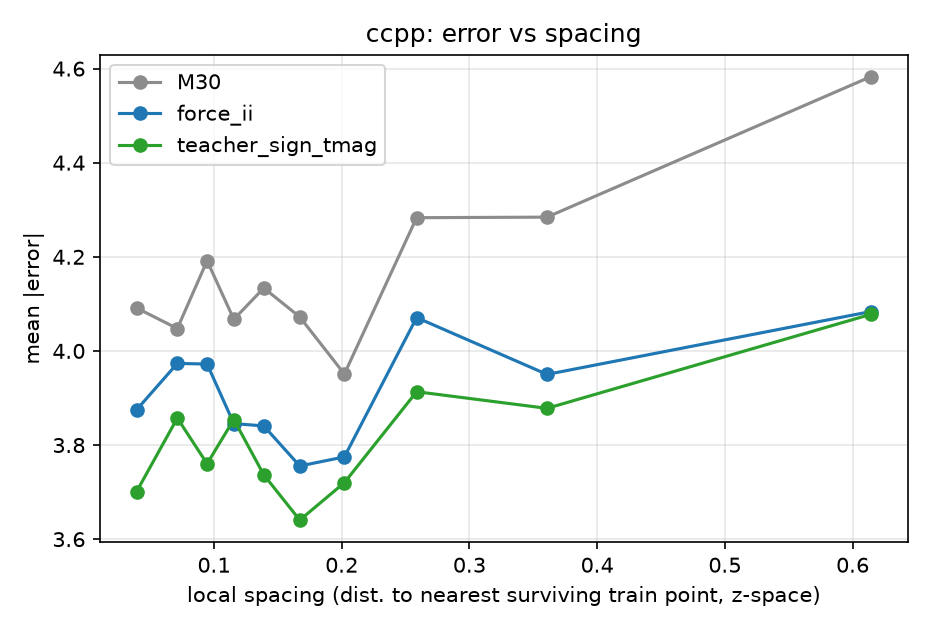
\includegraphics[width=.48\linewidth]{error_vs_spacing__ccpp.png}\hfill
%   
\includegraphics[width=.48\linewidth]{benefit_vs_spacing__ccpp.png}
%   \caption{Error (left) and benefit (right) vs.\ local spacing on ccpp.}
%   \label{fig:spacing}
% \end{figure*}

\section{Discussion: a unified mechanism}
\label{sec:discussion}

The two granularities combine into one account. \textbf{Distillation in RegressionTM is
predominantly a \emph{global reshaping} of the learned function, with a localized
hole-filling component that appears only for a sufficiently accurate teacher.}

This single mechanism resolves every recurring puzzle in the arc:

\begin{itemize}
  \item \textbf{Why teacher accuracy doesn't predict benefit
    (Section~\ref{sec:teacher_edge}):} the teacher having more data in the holes is
    largely irrelevant because its correction acts globally, not in the holes---except for
    the conditional B3 repair that only a good teacher can supply.
  \item \textbf{Why ``more data'' reasoning fails and ``less-is-more'' exists
    (Section~\ref{sec:full_data}):} learning quality is dominated by the dense bulk, where
    most points and most error mass live, not the sparse tail; adding harmful bulk points
    back can hurt without fixing the tail.
  \item \textbf{Why every mode is a sharpener, not a fixer
    (Sections~\ref{sec:sharpener}--\ref{sec:stability}):} a global reshaping scales
    whatever global signal the teacher carries and has no spatial mechanism to selectively
    repair weak regions.
  \item \textbf{Why spacing predicts benefit negatively
    (Section~\ref{sec:spacing}):} when a dataset's error is spacing-governed
    (heterogeneous), a single global correction mismatches the varying local structure and
    fails; when error is homogeneous, a global correction fits.
\end{itemize}

Spacing thus governs \emph{absolute difficulty} (B1) and \emph{which datasets benefit}
(Tier~A), but not \emph{where within a dataset distillation acts} (B2)---the difficulty
axis and the benefit axis are decoupled, joined only by the conditional, good-teacher
hole-filling of B3.

Throughout, the clause-level feedback of the TM was not merely the substrate but the
\emph{instrument}: because guidance modifies the Type~I/II decision directly, we could
attribute the runaway instability to the unbounded feedback type, localize benefit to
carved regions, and reason about magnitude sourcing---all in terms of the model's own
interpretable machinery.

\section{Limitations and Future Work}
\label{sec:limitations}

\subsection{Limitations}

\paragraph{Statistical power and panel size.}
The per-region analysis rests on four anchor datasets, and energy's spacing is partly
degenerate (discrete features collapse the deciles). The dataset-level correlations use
ten to twelve datasets with $p$-values uncorrected over many metric pairings, so some
associations partly reflect dataset size or dimensionality rather than spacing per se. The
strong, robust coupling is specifically \texttt{force\_ii\_tmag}; the other modes are
directionally consistent but weaker at this sample size. The teacher-edge correlations use
only the four anchor datasets and are not statistically significant. The ``less-is-more''
phenomenon is robust on just a few heterogeneous datasets (\texttt{nyse\_log},
\texttt{realestate}, \texttt{metro}); airquality's instance is seed-fragile and should not
be treated as canonical.

\paragraph{Protocol and configuration scope.}
All results are obtained within one masked-distillation protocol---nested structured
$k$-NN holes with a fixed teacher (80\% kept) and student (70\% kept)---so other scarcity
structures, mask fractions, or nesting depths may behave differently. The teacher is a
single frozen model rather than an ensemble, and the core hyperparameters ($T$, clause
count, specificity, blend factor $f$, teacher-firing probability $p_{\text{teacher}}$, and
epoch budget) are held fixed rather than swept, so the reported effect sizes are specific
to this operating point.

\paragraph{Mechanism and measurement scope.}
The mechanisms act on the per-sample error sign and magnitude; we did not explore
scheduling $p_{\text{teacher}}$ over training, per-region teacher trust, or combinations of
modes. Our spacing metrics are computed in input (feature) space, and \texttt{spc\_err\_strength}
is a derived heuristic rather than a first-principles quantity. Finally, while the
clause-level feedback makes the mechanism inspectable, our interpretability claims are
qualitative: we did not quantify which clauses or literals the teacher actually changes.

\subsection{Future Work}

Several directions follow directly from these limitations.

\begin{itemize}
  \item \textbf{Spacing definitions.} Separate input-space spacing from joint
    input--target $(x,y)$ spacing to pin down the operative variable, and compare
    alternative density and heterogeneity measures against \texttt{spc\_err\_strength}.
  \item \textbf{Broader, more rigorous evaluation.} Extend the panel and apply
    multiplicity-corrected statistics to test whether the density--benefit law holds
    across all modes, not only \texttt{force\_ii\_tmag}.
  \item \textbf{Scarcity structures.} Test random, adversarial, class-imbalanced, and
    out-of-support (extrapolation) holes, and vary the mask fraction and nesting depth, to
    map how the global-reshaping-plus-local-repair account depends on how data is removed.
  \item \textbf{Teacher design and gating.} Explore teacher ensembles, self-distillation,
    and iterative teacher--student rounds; and, since accuracy does not predict benefit,
    build a data-geometry gate---for example a spacing-based go/no-go rule---that decides
    when to distil at all.
  \item \textbf{Mechanism extensions.} Study scheduled or learned $p_{\text{teacher}}$,
    per-region teacher trust, and combinations of teacher-bounded magnitude with adaptive
    triggering, and port the mechanisms to the weighted and convolutional variants and to
    classification Tsetlin Machines.
  \item \textbf{Interpretability and theory.} Quantify what the teacher transfers at the
    clause level---turning the ``inspectable'' claim into measurements---and develop a
    theoretical account of why global reshaping dominates and when localized in-hole repair
    emerges from the Type~I/Type~II dynamics.
\end{itemize}

\section{Conclusion}
\label{sec:conclusion}

We studied teacher-guided knowledge distillation for the Regression Tsetlin Machine by
letting a frozen teacher steer the student's clause-level Type~I/II feedback, and asked
not only whether it helps but when, where, and why. Across a family of mechanisms and a
controlled masked-distillation benchmark, we found that every mechanism is a
\emph{sharpener} that scales the teacher's signal without rescuing a bad teacher; that
teacher accuracy does not predict benefit; that a 70\%-data guided student can reach and
occasionally exceed a full-data model; and that data spacing/density---not teacher
accuracy---governs distillation benefit. These consolidate into a single account:
distillation is a predominantly global reshaping of the learned function that helps when
a dataset's error is not spacing-governed and fails when it is, with a good teacher
additionally repairing the specific regions whose training support was removed. The
transparency of the TM's clause feedback was essential to reaching, and to explaining,
each of these conclusions.

\paragraph{Open threads.}
\begin{itemize}
  \item Distinguishing input-space spacing from joint $(x,y)$ spacing as the operative
    variable.
  \item Firming the per-dataset density$\leftrightarrow$benefit correlation for modes
    other than \texttt{force\_ii\_tmag}, where it is currently weaker.
  \item Testing the account under non-structured (e.g.\ random or adversarial) scarcity
    patterns.
\end{itemize}


\bibliographystyle{IEEEtran}
\bibliography{references}

\end{document}
